\chapter{Architektura}
\label{ch:funplenop}

W tym rozdziale zostanie omówiona część projektu związana z architekturą oraz środowiskiem pracy

\section{Wiodąca technologia}

% Graphics which gives us with Native(IOS, Android), React-Native (IOS, Android, React-Native), WebApp (React)

Podczas wyboru wiodącej technologii w projekcie brałem pod uwagę głównie kwestię szybkości dostępu do aplikacji dla użytkowników oraz możliwość jej obsługi na wielu urządzeniach naraz w tym jako aplikacja dektopowa, mobilna na system IOS oraz Android. Tym samym ze względu na rozbudowaną i rozproszoną architekturę zależało mi na jednolitej technologii.

\subsection{Możliwości}
Rozważając decyzję wyboru głównej technologii brałem pod uwagę 3 możliwości.
\begin{itemize}
    \item \textbf {Aplikacje mobilne w natywnych technologiach} \\
        Wybór budowy natywnych aplikacji mobilnych wiązał by się z tym, że aby utrzymać aplikację dla systemu IOS, Android oraz wersję desktopową wystąpiła by potrzeba utrzymywania systemu w kilku różnych językach programowania co znacznie mogłoby obniżyć jakość kodu oraz utrudnić realizację projektu oraz jego dalsze utrzymywanie. Inną wadą tego rozwiązania byłoby płatne i skomplikowane publikacje aplikacji mobilnych. Ostatnim oraz najważniejszym czynnikiem pominięcia wyboru tego rozwiązania było wymagany czas i miejsce w urządzeniu na aplikacje. Ideą aplikacji jest możliwość jej szybkiej instalacji stąd też na podstawie innych znalezionych rozwiązań, to zostało zdysklasyfikowane mimo możliwości zapewnienia wszystkich natywnych funkcjonalności

    \item \textbf {Aplikacje mobilne napisane w React Native} \\
        React Native to technologia opracowana przez firmę Facebook w celu przyśpieszenia procesu tworzenia aplikacji mobilnych.Pozwala ona na jednoczesne budowanie aplikacji zarówno na system IOS oraz Android w języku JavaScript. Mimo zoptymalizowanego procesu budowania aplikacji mobilnych nadal wedle założeń projektu potrzebne jest zbudowanie aplikacji desktopowej. Tym samym proces publikacji aplikacji pozostaje dokładnie taki sam jak w 1 możliwości, budowy aplikacji w technologiach natywnych.
    \item \textbf {Aplikacja internetowa SPA oraz PWA} \\
        Ostatnią możliwością była aplikacja internetowa typu SPA (Odwołanie) oraz PWA (Odwołanie). Takie podejście umożliwia budowę szybkiej oraz wieloplatformowej aplikacji w jednolitej technologii oraz architekturze. Użytkownicy posiadają dostęp do strony internetowej, która może zostać zainstalowana na każdym telefonie oraz komputerze zacznie szybciej oraz zajmując mniejszą ilość na urządzeniu niż w przypadku natywnych technologii. Mimo ograniczenia niektórych funkcjonalności, szczególnie na telefonach z systemem IOS względem natywnych rozwiązań wybrane podejście oferuje funkcjonalności potrzebne do budowy projektu. Kolejną rzeczą, która zadecydowała o wyborze był proces publikacji aplikacji. Rozwiązanie to pozwala na jednoczesną, prostą i bezpieczną publikację w jednolitym systemie.
\end{itemize}

\subsection{Wybór}
Ze względu na szybkość dostępu, łatwość instalacji z punktu widzenia użytkowników, jednolitą technologię dla wielu platform oraz prostszy w porównaniu z pozostałymi możliwościami proces publikacji, ostatecznym wyborem pozostała aplikacja internetowa typu SPA oraz PWA.

\section{JavaScript}
% https://developer.mozilla.org/pl/docs/Learn/Getting_started_with_the_web/JavaScript_basics
% https://pl.wikipedia.org/wiki/JavaScript
% https://babeljs.io/

Jako główny język programowania wykorzystany do implementacji tego projektu został zastosowany JavaScript. Ze względu na swoje możliwości oraz szeroką grupę społeczności umożliwia on jednoczesną budowę wszystkich części projektu (klient, serwer, raspberry pi).
\\\\
JavaScript (JS) jest skryptowym oraz dynamicznym językiem programowania wysokiego poziomu stworzony przez firmę Netscape. Jego bezpośrednim twórcą jest amerykański programista Brendan Eich. JavaScript jest wieloparadygmatowym językiem programowania co oznacza, że można w nim programować zarówno obiektowo, funkcyjnie jak i imperatywnie. Wersje JavaScriptu rozpoznawane są względem standardu specyfiki ECMAScript wydaną przez organizację ECMA. Obecnie rozwojem tego standardu zajmuje się komicja TC39, która zrzesza przedstawicieli wszystkich głównych przeglądarek internetowych.
\\\\
Ważnym aspektem wersji tego języka jest jego wspieranie w różnych przeglądarkach. Tworząc nowy projekt chcemy korzystać zazwyczaj z najnowszych implementacji przy jednoczesnej obsłudze w różnych przeglądarkach i ich różnych wersjach. Jak rozwiązanie tego problemu powstał darmowy i otwarty transpilator JavaScriptu. Umożliwia on konwersję z najnowszych wersji JS do tego zgodnego z ES5 (wersja JS z 2009 roku przyjęta jako minimalny standard użycia).

\section{Stos technologiczny}
Na podstawie wybranego podejścia budowy aplikacji oraz języku programowania musiałem określić stos technologiczny wykorzystywany w projekcie.
Ze względu na zakres projektu i cel zapewnienia jak najprostszej dalszej rozbudowy projektu oraz moje doświadczenie komercyjne w budowaniu aplikacji internetowej zdecydowałem się wybrać stos technologiczny zwany MERN (Mongo-Express-React-Node). W poniższych sekcjach rozwinę zagadnienia związane z każdą z tych technologii oraz przeanalizuję podjęty wybór na tle innych alternatyw.

\section{Diagramy}

\begin{tabular}{c}
    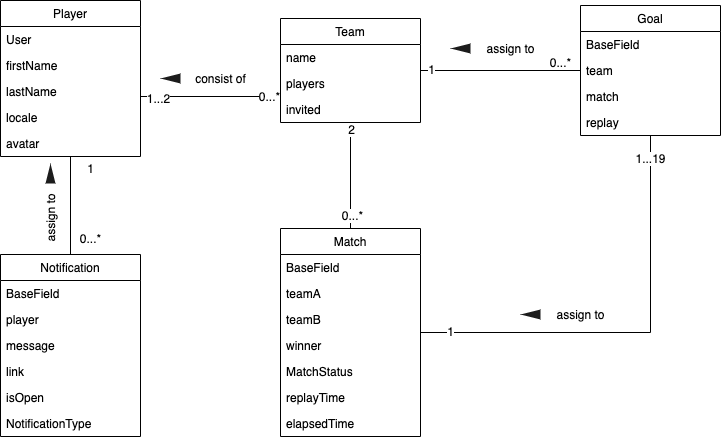
\includegraphics[width=\textwidth]{images/diagrams/class_diagram.png}  \\
    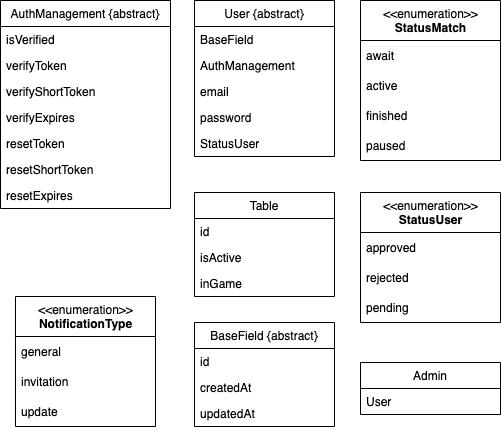
\includegraphics[width=\textwidth]{images/diagrams/class_diagram_rest.png}
\end{tabular}

\begin{figure}[h!]
  \centering
    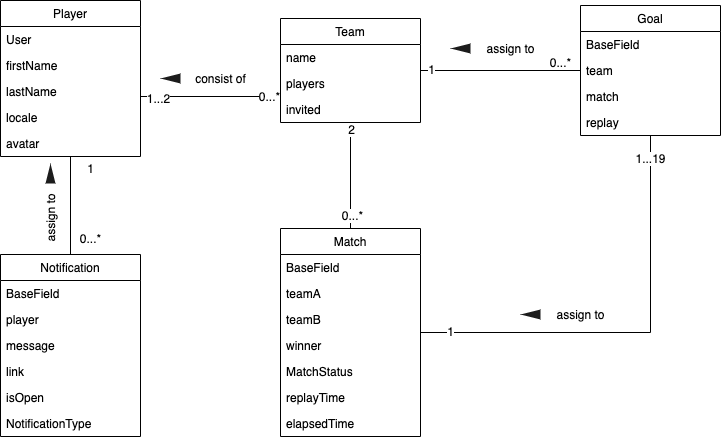
\includegraphics[width=0.5\textwidth]{images/diagrams/class_diagram.png}
  \caption{Diagram klas}
  \label{fig:mobile}
\end{figure}

\begin{figure}[h!]
  \centering
    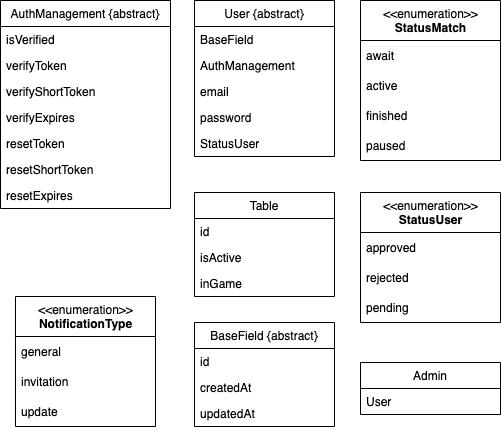
\includegraphics[width=0.5\textwidth]{images/diagrams/class_diagram_rest.png}
  \caption{Digram klas bez relacji}
  \label{fig:mobile}
\end{figure}

\begin{figure}[h!]
  \centering
    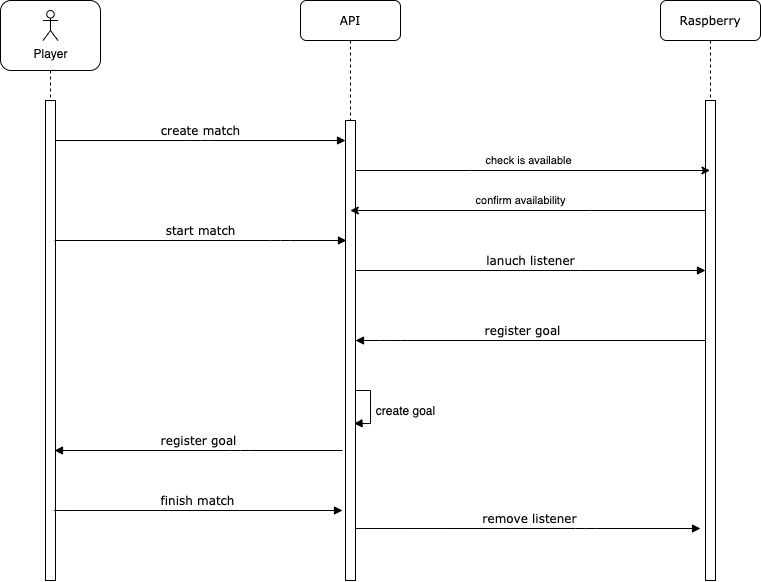
\includegraphics[width=0.5\textwidth]{images/diagrams/match_event_flow.png}
  \caption{Digram sekwencji dla działania stołu}
  \label{fig:mobile}
\end{figure}

\section{Struktura projektu}
Ze względu na fakt budowy wielu serwisów, które mogą dzielić między sobą zasoby oraz potrzebują siebie nawzajem do prawidłowego działania potrzebowałem narzędzia, które umożliwi mi dynamiczną pracę miedzy serwisami. Podczas planowania struktury i przyszłego zarządzania projektem brałem pod uwagę 3 podejścia. W każdym z przedstawionym przykładzie zakładam korzystanie z git'a oraz menadżera zależności Yarn.

\begin{itemize}
    \item \textbf {Osobne repozytoria z wykorzystaniem yarn link} \\
        Pierwszym rozważanym podejściem było stworzenie osobnych repozytoriów dla każdego serwisu.
        Umożliwiłoby to zachowanie klarownej historii repozytorium dla każdego serwisu. W przypadku osobnych repozytoriów, korzystanie przez siebie nawzajem byłoby możliwe z wykorzystaniem komendy `yarn link` między serwisami. Takie rozwiązanie jednakże byłoby problematyczne przy pracy ze względu na ilość serwisów oraz dlatego, że komendę odpowiadającą za linkowanie między serwisami trzeba byłoby wpisywać z każdą reinstalacją zależności w serwisach. Innym problem dla takiego podejścia byłaby konfiguracja narzędzi takich jak linter czy prettier, ponieważ ich konfiguracje musiałyby się znaleźć w każdym z repozytorium a zmiany wprowadzone w jednym miesjcu trzeba byłoby nanosić manualnie w innych miejscach.

    \item \textbf {Osobne repozytoria z wykorzystaniem git submodules} \\
        Innym podobnym rozwiązaniem do tego powyższego byłoby zastosowanie git submodules. Umożliwiłoby to Utrzymywanie każdego serwisu w osobnym repozytorium ale całość połączona miałaby swoje repozytorium z odnośnikami do poszczególnych repozytoriów. Rozwiązałoby to kwestie globalnej konfiguracji narzędzi takich jak linter ale nadal pozostałby problem z wzajemnym linkowaniem między serwisami.

    \item \textbf {Mono repozytorium z wykorzystaniem yarn workspaces} \\
        Ostatnią rozważaną możliwość było podejście budowy projektu jako jedno monolityczne repozytorium. To rozwiązanie wprowadza pojęcie paczek, które w powyższych opcjach byłyby osobnymi repozytoriami. Dzięki takiemu podejściu możemy przechowywać cały projekt w jednym repozytorium, jednakże zmniejsza to czytelność historii commitów repozytorium. Mimo wymienionej wady zarządzanie oraz korzystanie z projektu w tym przypadku może być znacznie prostsze. Korzystając z workspace'ów wszystkie paczki mogą bez żadnej dodatkowej konfiguracji korzystać z siebie nawzajem. Poza tym globalna konfiguracja narzędzi takich jak linter jest możliwa dla wszystkich paczek.

\end{itemize}

Ostatecznym wyborem pozostało podejście budowy projektu w architekturze monolitycznego repozytorium korzystając z yarn workspaces.

\section{Typy}
Język JavaScript jest jezykiem programowania, który nie jest silnie typowany. Ze względu na rozmiar całego systemu oraz brak moliwości typowania w wybranym jezyku programowania, została przygotowana paczka 'core', która podzielona jest na 2 części, modele oraz stałe.
Dzięki takiemu rozwiązaniu zostało wprowadzone ręcznę typowanie części logiki biznesowej całego systemu oraz stałych zmiennych wykorzystywanych we wszystkich pakietach poprzez zwykłe obiekty. 

Innym narzędziem rozwiązującym problem braku typowania jest paczka 'Prop Types' pochodząca od twórców biblioteki 'React'. W projekcie wykorzystywana jest w pakietach 'player', 'admin' oraz 'ui-components'. Jej zadaniem jest kontrola typów przyjmowanych argumentów w komponentach graficznych.

Dzięki dwóm powyszym rozwiązaniom budowa aplikacji posiadała rodzaj mechanizmu typowania. Przyczyniło się to do szybszego procesu pracy oraz zminiejszyło ilość potencjalnych błędów w systemie.

\section{Środowisko developerskie}
Podczas wyboru technologii oraz narzędzi do pracy bardzo ważnym etapem był dobór środowiska developerskiego. Przez środowisko developerskie rozumiane są narzędzia służące ogólnej pracy nad programistyczną częścią systemu, zwiększeniu jej bezpieczeństwa oraz jej przyśpieszenia.

\subsubsection{Edytor kodu}

\subsubsection{Menażdżer Wersji Node.js}

\subsubsection{Lintery}

- Eslint \& Prettier \& commitlint \& sort package json
- husky \& lint staged

\subsubsection{Zarządzanie monorepozytorium}

\subsubsection{Zarządzanie wersją}

\subsubsection{Zdalne repozytorium}

- webstorm/vscode
- NVM

- Lerna



\section{Github i Git}
- Zdalne repozytorium (github vs rest)
- Wersje
- Git hooki
